\documentclass[notitlepage,12pt]{report}
\usepackage[left=1in, right=1in, top=1in, bottom=1in]{geometry}

\usepackage{titling}
\usepackage{lipsum}
\usepackage{braket}
\usepackage{graphicx}
\usepackage[table]{xcolor}
\graphicspath{./images/}
\usepackage{subcaption}
\newcommand{\tr}{\mathrm{tr}}
\usepackage{hyperref}
\usepackage{authblk}
\usepackage[backend=biber, style=chem-acs]{biblatex}
\usepackage{tabularx}
% \usepackage{amsmath}
\usepackage{mathtools}% Loads amsmath
\usepackage{physics}
\renewcommand\thesection{\arabic{section}}

\bibliography{bib}
\addbibresource{bib.bib}


\begin{document}
	\title{Electronic properties in condensed-phase molecular systems under Embedded theoretical approaches: Liquid water systems}
	\author[1]{Jessica Martinez}
	\affil[1]{Department of Chemistry, Rutgers University, Newark, New Jersey}
	\date{June 2022}
	\renewcommand\Affilfont{\itshape\small}
	\thispagestyle{empty}
\maketitle
\section{Introduction}

	High accurate description at the electronic level in condensed-phase molecular systems (CPMS) as liquid water requires a perfect equilibrium between the use of spectroscopy techniques\supercite{reimann2021two,malerz2021low,bolognesi2021combined} and computational approaches \supercite{couto2007understanding,ambrosio2016structural,ozaki2021advances}. Two important properties widely used in liquid water characterization imply the determination of the Ionization Potentials (IPs)\supercite{thurmer2021accurate,perry2020ionization,credidio2021quantitative,thurmer2021valence,tolle2019charged,gaiduk2018electron,gaiduk2016photoelectron,seidel2016valence}, as well as, the core electronic excitations to the continuous\supercite{zhovtobriukh2019liquid,zhang2020isotope,smith2020femtosecond}.
	
	On one side, the determination of IPs of liquid water, which implies the knowledge of the ionized states of the electrons, take part in many crucial processes in electrochemistry\supercite{marenich2014computational}, photochemistry\supercite{reuther1996primary,hu2021photochemical} as well as peculiar states of matter like excess electrons solvated in liquid water\supercite{ambrosio2017electronic}. 
	
	Recent advances in liquid microjet (LJ) photoelectron spectroscopy have opened the door to the determination of accurate electronic energetics of water and aqueous solutions \supercite{thurmer2021accurate,perry2020ionization,credidio2021quantitative,thurmer2021valence}. Perry \textit{et al}. \supercite{perry2020ionization} obtained values for the vertical and adiabatic ionization energies (which are indicated by VIE and AIE, respectively) of liquid water of 11.67 and 10.12 eV, regarding the $1b_1$ orbital band.   A second study determined a more accurate value for the VIE of liquid water of 11.33 $\pm$ 0.03 eV accounting for a critical factor: the measuring of the liquid-phase low-energy cutoff spectrum along with the photoelectron peak of the interest in up to a broad range of photon energies (15-950 eV)\supercite{thurmer2021accurate}.
	
	From the theoretical side, Gaiduk \textit{et al.} \supercite{gaiduk2018electron} employed path-integral molecular dynamics (PIMD) with \textit{ab-initio} potentials in combination with many-body perturbation theory (MBPT) within the $G_{0}W_{0}$ approximation starting from a range-separate hybrid (RSH) for the description of the ground-state for liquid water. Their values for the AIE and VIE  are 10.26 and 11.53 eV, respectively.  Similarly, Ziaei \textit{et al}. \supercite{ziaei2018probing} utilized a self-consistent GW approach with a vertex correction and the projector augmented wave (PAW) method \supercite{dal2014pseudopotentials} finding  good agreement with the results of Gaiduk \textit{et al.} \supercite{gaiduk2018electron}. Both results are remarkable in that they reproduce the experiment to within a few tenths of eVs.
	
	Following the trend but now employing   Density Functional Theory (DFT) \supercite{thomas1927calculation,fermi1927statistical, hogenberg, kohn}, a theory based on the electron density rather than many-body wavefunctions, a previous work\supercite{tolle2019charged} attempted the calculation of IPs of liquid water based on a new subsystem DFT method\supercite{jacob2014subsystem,wesolowski2015frozen,krishtal2015subsystem} capable of approaching charged systems regardless of the underlying adoption of periodic boundary conditions with simulation cells containing a constrained number of molecules \supercite{tolle2019charged}, called “Impurity Model”. 
	
	In detail, subsystem DFT ameliorates the limitation of DFT in the studying of bulk systems as liquids i.e., an infinite number of molecules, based on a divide-and-conquer strategy. In which the total electron density is divided into a sum of individual densities, which effectively scales almost linearly concerning the system size, called subsystem DFT or Frozen Density Embedding (FDE) \supercite{mi2021eqe,mi2019nonlocal,mi2019ab}. By partitioning a bulk-phase system into smaller subsystems allows the selection of a few or even one subsystem of interest, which as a consequence is embedded in a complex environment \supercite{schmitt2020frozen}. This arises to a robust strategy to study the effects of the environment due to a single subsystem, the so-called “Embedding Potential” \supercite{genova2016avoiding}. 
	
	The “Impurity Model” relies on the fact that Coulomb potentials for the electronic and nuclear charges can be computed based on a Screening potential. This Screening potential arises for the contribution of the “Embedding potential” of the periodic images with respect to the same subsystem, which generates a partition of the system into a finite, nonperiodic subsystem with density $\rho_I$, and a semi-infinite environment. The above can be done because a subsystem’s electron density can be taken for the density of an extended, periodic subsystem or the density of a finite, single subsystem. Details are found in the reference paper\cite{tolle2019charged}. 
	
	Based on both  the “Impurity Model” and adding the $\Delta$-SCF approach\supercite{bagus1965self,waskom2017mwaskom} (the energy difference between the neutral and the polarized systems) not only the vertical IP of liquid water are computed, but also a breakdown of the IP into five contributions is obtained:  (1) \textbf{Mean field}: the ionization energy of each water molecule computed at the mean-field, Hartree-Fock level; (2) \textbf{Correlation}: the effect of going beyond Hartree-Fock to account for electron correlation within each water molecule at the correlated wavefunction level as well as DFT; (3) \textbf{Interaction}: interaction with the environment which consist of the Coulomb interactions between each water molecule and their environment (an infinite bulk of liquid water) augmented by effects of exchange, correlation and Pauli repulsion (non-additive kinetic energy); (4) \textbf{Polarization}: polarization of the environment electronic structure in response to the ionization of a nearby water molecule; and finally, (5) \textbf{Delocalization}: the possibility that the spin density of the cation is delocalized over more than one water molecule.
	
	For this work, the IP was determined by averaging over 128 multiple snapshots of 64 water molecules considered in the corresponding simulation cell. Two \textit{ab-initio} molecular dynamics (AIMD) trajectories were used separately, a Born-Oppenheimer(BO) trajectory and a path-integral(PI) dynamics trajectory \supercite{gaiduk2018electron}. The average mean-field contribution is then successfully obtained over the 64 subsystems (av. 10.81 eV) and reformed by three essential corrections: Correlation, Interaction, and Polarization, which implies the inclusion of electronic and environmental contributions to surpass the Hartree-Fock limitations. 
	
\begin{minipage}{0.4\textwidth}
	\label{cont_ip}
	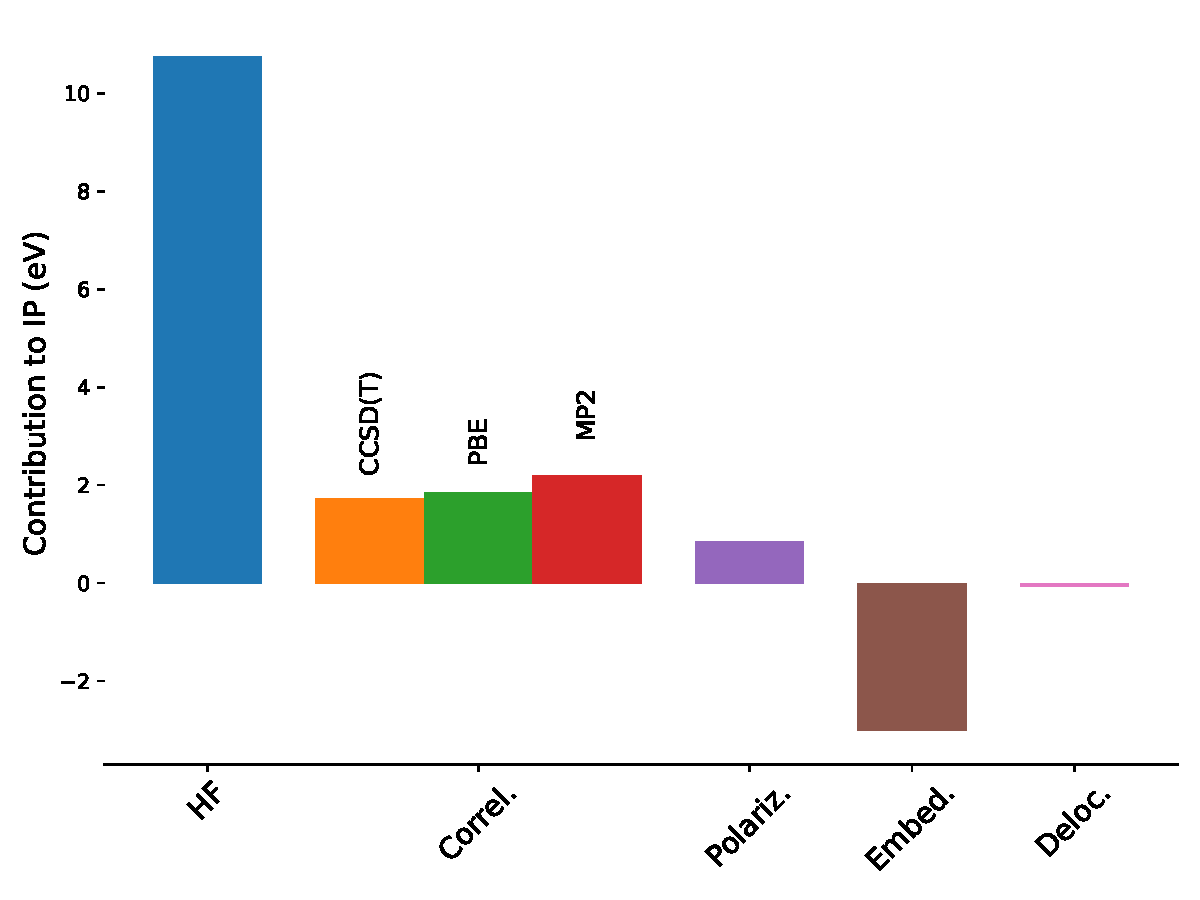
\includegraphics[width=\linewidth]{./images/contribution_liquidwater_PI}
	{Contribution chart for the first 10 snapshots form PI dynamics trajectory. \supercite{gaiduk2018electron}}
\end{minipage}
\begin{minipage}{0.55\textwidth}
	In terms of the correlation, we found a consistent trend among CCSD(T), PBE, and MP2 methods, see Figure \ref{cont_ip}, with a slight overestimation of av. 0.28 eV for MP2, compared with one of the most accurate treatments of the electronic correlation, CCSD(T). The polarization of the electronic environment nearby an ionized water molecule arises with a correction average of av. 0.84 eV while the embedding correction subtracts av. -2.80 eV for both PI and BO systems. Subsequently, a fifth contribution was found to have a negligible effect, namely, accounting for spin density delocalization over more than one water molecule. 
\end{minipage}
	
	Going beyond FDE, an alternative embedding approach connecting subsystem DFT emerged, the so-called block-orthogonalized Manby-Miller embedding (BOMME). BOMME is a projection operator technique that is forgoing the use of approximate KEDFs and allows the fragmentation of a system through covalent bonds\supercite{ding2017embedded}. BOMME with a combination of real-time TDDFT (rt-BOMME) has presented a better performance in the capture of both intermolecular and intramolecular coupling among subsystems \supercite{koh2017accelerating}.
	
	On the other hand, with the interest of characterizing the core electronic excitations to the continuous, X-ray absorption near-edge structures (XANES) spectrum also plays an important role. X-ray absorption spectroscopy (XAS) targets the study of excitation from core orbitals due to absorbing photons in the X-ray energy range\supercite{fransson2016x}. XANES features three zones K-edge, $L_1$-edge, and $L_2$-edge, which allow the study of the oxidation state, local symmetry, and coordination environment in gas, liquid, or solid phase\supercite{rehr2005progress,koningsberger1987x}. 
	
	Particularly, for the simulation of XAS in liquids multiple theoretical approaches have came up, Transition potential(TP)-DFT \supercite{triguero1998calculations}, TDDFT employing Davidson procedure\supercite{davidson197514}, Excited-state core hole (XCH)\supercite{prendergast2006x}, Bethe-Salpeter equation (BSE) and Hedin’s GW approximation of the quasiparticle \supercite{vinson2012theoretical}, Coulomb hole and screened exchange (COHSEX)\supercite{chen2010x}, and QM/MM techniques\supercite{list2014lanczos}. A detailed description of each approach is found in the review \cite{fransson2016x}. 
	
	In summary, these approaches’ main failures range from the only qualitative prediction of the experiment (TP-DFT), the well-known self-interaction error leading to an underestimation of core-excitation energies (TDDFT), as well as the use of small unit cells that narrow the post-edge region(XCH). Following the same trend due to over-structured clusters, there is an overestimation of the post-edge intensity and an underestimation of the post-edge energy (COHSEX). An overestimation of the main edge is also visible using a small number of molecules (BSE). Finally, disregarding significant orbital rehybridization effects due to the classical treatment of surrounding molecules (QM/MM) also misled the XAS spectrum’s prediction.
	
	In this work, taking advantage of the newest implementation of rt-BOMME and rt-sDFT \supercite{de2021environment} in Psi4 code \supercite{smith2020psi4}, to predict and overcome the already mentioned failures in the modeling of the X-ray absorption near-edge structures (XANES), we wish to go further in applications of the method for more significant systems than the first solvation shell of Cl and F in water (counting for eight water molecules). To accomplish this, we selected three main clusters (1) Liquid water and Ice, (2) Cations solvated in water, and (3) A complex molecule ($K_3[Fe(CN)_6]$) solvated in water. Additionally, a previous implementation of rt-sDFT in ADF\supercite{te2001chemistry} and eDFTpy\supercite{edftpy}, code-based of Quantum espresso package\supercite{giannozzi2009quantum}, will be used.


\section{Theoretical Background}

	\subsection{Subsystem DFT}
	Subsystem DFT or Frozen Density embedding formalism developed by Wesolowski and Warshel employs a divide-and-conquer approach where the Kohn--Sham (KS) problem is solved for fragments of small size, the so-called subsystems, which alleviate the $n^3$ scaling of KS-DFT\supercite{sDFT,wesolowski1993frozen,wesolowski2006one}. In subsystem-DFT the electron density of the total system $\rho$ is partitioned into subsystem electron densities and can be written as

	\begin{equation}\label{eq:sumdensity}
		\rho(r) = \sum\limits_{I=1}^{ \# \ of \ subsystems} \rho_{I}(r),
	\end{equation}

	where the index $I$ runs over all the subsystems.
	
	The subsystem densities $\rho_I$ are constructed from the absolute square of all subsystem-specific orbitals $\psi_{i}^I(r)$ as

	\begin{equation}\label{eq:subso}
		\rho_I( r) = \sum\limits_{i=1}^{n_I} \abs{\psi_{i}^I(r)}^2,
	\end{equation}
	
	where $n_I$ accounts for the total number of electrons per subsystem $I$.
	The total electronic energy becomes a function of all the subsystem densities and has the form,

	\begin{equation}
		E[\{\rho_I\}] = \sum\limits_I T_{s}[\rho_I] + V_{\mathrm{nuc}}[\rho] + E_H[\rho] + E_{\mathrm{xc}}[\rho] + T_{s}^{\mathrm{nad}}[\{\rho_I\}],
	\end{equation}
	
	where $V_{\mathrm{nuc}}[\rho]=\int \rho(r) v_\mathrm{ext}(r)dr$, and $E_H[\rho]$ and $E_{\mathrm{xc}}[\rho]$ are the Hartree  and exchange-correlation energy functionals.
	
	Conventionally, the sum of the single subsystem kinetic energy contributions $T_s[\rho_I]$ is not equal to the total non-interacting kinetic energy of the system. In such a way, a non-additive contribution arises, which is captured by the non-additive kinetic energy functional (NAKE), defined as

	\begin{equation}
		\label{nad}
		T_{s}^{\mathrm{nad}}[\{\rho_{I}\}] = T_{s}[\rho] - \sum\limits_{I=1}^{N_S} T_{s}[\rho_{I}].
	\end{equation}

	The variational problem is cleared up by solving self-consistently a KS like equation per subsystem with constrained electron density \supercite{wesolowski1994ab}, which reads

	\begin{equation}\label{eq:ksced}
		\left( -\frac{\nabla^2}{2} + v_{\mathrm{eff}}^{I}[\rho_I](r) + v_{\mathrm{emb}}^{I}[\rho_{I},\rho](r) \right) \psi_{i}^I(r) = \epsilon_{i}^I \psi_{i}^I(r)
	\end{equation}
	The subsystem orbital energies are denoted by $\epsilon_{i}^I$ in Eq.\ \ref{eq:ksced}.\supercite{sDFT}, and the subsystem effective KS potential ($v_{\mathrm{eff}}^{I}[\rho_I](r)$) is defined as

	\begin{equation}\label{equ6}
		v_{\mathrm{eff}}^{I}[\rho_I](r) = v_{\mathrm{ext}}^I(r) + v_{{H}}[\rho_I](r) + v_{\mathrm{xc}}[\rho_I](r).
	\end{equation}

	In equation \ref{equ6},  $v_{\mathrm{ext}}^I(r)$ is the  external potential of subsystem $I$ while $v_{\mathrm{H}}[\rho_I](r)$ and $v_{\mathrm{xc}}[\rho_I](r)$ represent the Hartree and the exchange-correlation potentials per subsystem $I$.

	By way of explanation, the Kohn–Sham single-particle Hamiltonian is augmented by an embedding potential, in which  are encoded the interaction of the electrons of subsystem $I$ with the environment, which reads as follows,

	\begin{equation}\label{embedd}
		\begin{aligned}
			v_{\mathrm{emb}}^{I}[\rho,\rho_I](r) = \sum\limits_{J,J \neq I} &v_{\mathrm{ext}}^{\; J}(r) + v_{{H}}[\rho - \rho_I](r)  \\ + \ &v_{\mathrm{xc}}^{\mathrm{nad}}[\rho,\rho_{I}](r) + v_{T_s}^{\mathrm{nad}}[\rho,\rho_{I}](r),
		\end{aligned}
	\end{equation}
	where $v_{\mathrm{ext}}^{\; J}$ and $v_{{H}}[\rho - \rho_I](r)$ are the inter-subsystem potentials that capture the Coulomb interactions. In detail, the non-additive exchange-correlation and kinetic potential of the environment $v_{\mathrm{xc}}^{\mathrm{nad}}[\rho,\rho_{I}](r)$ is defined as
	
	\begin{equation}
		\label{emb_xct}
		v_{\mathrm{xc, T_{S}}}^{\mathrm{nad}}[\rho,\rho_{I}](r) = \frac{\delta E_{\mathrm{xc, T_{S}}}[\rho]}{\delta \rho(r)} - \frac{\delta E_{\mathrm{xc, T_{S}}}[\rho_I]}{\delta \rho_I(r)}.
	\end{equation}

	In practice, this set of equations can either be solved iteratively using  a Freeze-and-Thaw\supercite{FaT} procedure(as done in ADF\supercite{te2001chemistry} and other molecular codes), or simultaneously by all subsystems where the total density is updated at every SCF cycle (as done in CP2K \supercite{hutter2014cp2k} and Quantum-Espresso\supercite{RN48,mi2021eqe}).

\subsection{rt-TDDFT}


\subsection{BOMME}

\section{Computational Details}

	Embedding potentials are obtained by equation \ref{embedd} following the frozen density embedding (FDE) method \ref{eq:ksced} implemented in the embedding Quantum Espresso (eQE) package \supercite{genova2017eqe}- Ultrasoft pseudopotentials from the PSL pseudopotential library \supercite{corso2014comput} are employed. 
	
	Embedding potentials from eQE are on regular fast Fourier transform (FFT) grid which are further fitted to smooth custom grids using an atom-centered grid function in eQE \supercite{genova2017eqe} and PySCF \supercite{PYSCF}. The above, allows the use of the Embedding potentials in molecular-based codes for a self-consistent field(SCF)\supercite{purvis1976transition} ground state total energy determination. 

\section{Current project and future directions}


\section{Conclusions}

\printbibliography

\end{document}
